\documentclass[tikz,border=8pt]{standalone}
% Shared look for every TikZ diagram. Load with \input{../../tools/tikz-style.tex}
\usepackage[sfdefault]{roboto}
\usetikzlibrary{arrows.meta, positioning, shapes.geometric, calc, fit, backgrounds}
\definecolor{cblue}{HTML}{4C78A8}
\definecolor{corange}{HTML}{F58518}
\definecolor{cgreen}{HTML}{54A24B}
\definecolor{cred}{HTML}{E45756}
\definecolor{cpurple}{HTML}{B279A2}
\definecolor{cgrey}{HTML}{6B6B6B}
\tikzset{
  every picture/.style={font=\sffamily, line width=1.2pt},
  box/.style={draw=#1, fill=#1!12, rounded corners=4pt, align=center, inner sep=7pt, minimum height=1.1cm},
  box/.default=cgrey,
  arrow/.style={-{Stealth[length=3mm]}, draw=cgrey, line width=1.4pt},
  title/.style={font=\sffamily\bfseries\Large},
  note/.style={font=\sffamily\small, text=cgrey, align=center},
}
\AtBeginDocument{\hyphenpenalty=10000 \exhyphenpenalty=10000}

% The planning hierarchy of a self-driving car (Geiger L12 slides 7-11, after Paden et al. 2016): each layer turns
% the layer above's output into a more detailed one, from the destination down to steering, throttle and brake.
\begin{document}
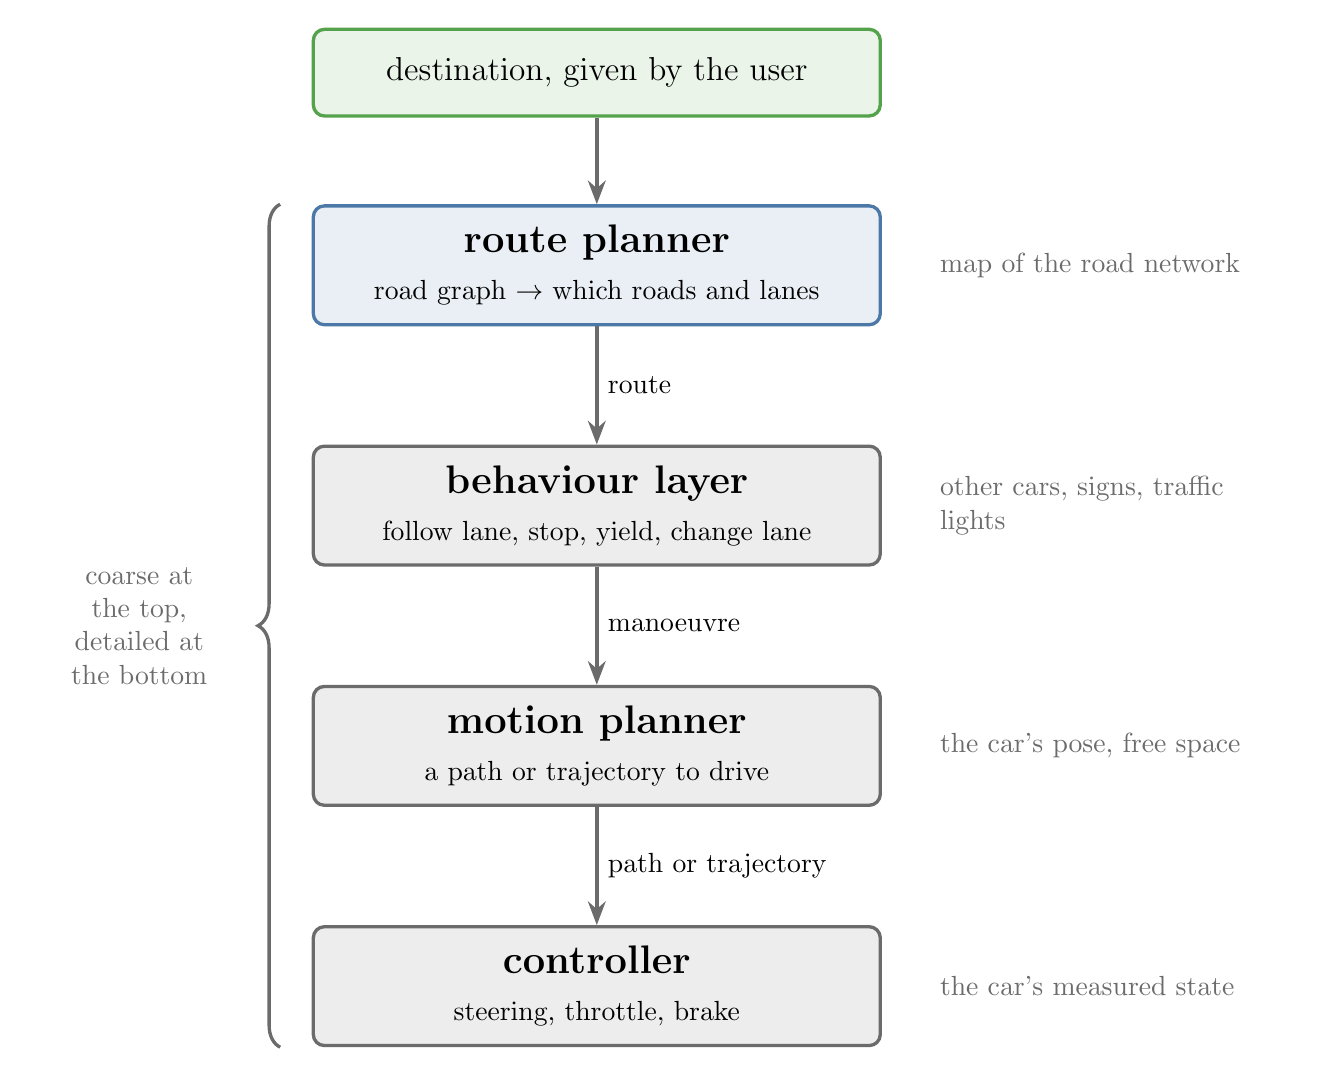
\begin{tikzpicture}[every node/.append style={font=\large}, node distance=1.5cm,
  lay/.style={box=#1, minimum width=7.2cm, minimum height=1.35cm, font=\Large},
  inp/.style={note, font=\normalsize, text width=4.4cm, align=left}]
  \node[lay=cblue] (r) {\textbf{route planner}\\[-1pt]{\normalsize road graph $\rightarrow$ which roads and lanes}};
  \node[lay=cgrey, below=of r] (b) {\textbf{behaviour layer}\\[-1pt]{\normalsize follow lane, stop, yield, change lane}};
  \node[lay=cgrey, below=of b] (m) {\textbf{motion planner}\\[-1pt]{\normalsize a path or trajectory to drive}};
  \node[lay=cgrey, below=of m] (c) {\textbf{controller}\\[-1pt]{\normalsize steering, throttle, brake}};
  \node[box=cgreen, above=1.1cm of r, minimum width=7.2cm] (d) {destination, given by the user};
  \draw[arrow] (d) -- (r);
  \draw[arrow] (r) -- node[right, font=\normalsize] {route} (b);
  \draw[arrow] (b) -- node[right, font=\normalsize] {manoeuvre} (m);
  \draw[arrow] (m) -- node[right, font=\normalsize] {path or trajectory} (c);
  \node[inp, right=0.6cm of r] {map of the road network};
  \node[inp, right=0.6cm of b] {other cars, signs, traffic lights};
  \node[inp, right=0.6cm of m] {the car's pose, free space};
  \node[inp, right=0.6cm of c] {the car's measured state};
  \draw[decorate, decoration={brace, amplitude=8pt}, cgrey] ([xshift=-0.4cm]c.south west) -- ([xshift=-0.4cm]r.north west)
    node[midway, left=10pt, note, font=\normalsize, text width=2.6cm, align=center] {coarse at the top,\\ detailed at the bottom};
\end{tikzpicture}
\end{document}
